\section{Introduction}
\label{sec:introduction}

Satellite--ground scheduling allocates contact opportunities that compete
for satellite and ground-station resources. When contacts belong to
different agents, replacing one agent's commitments can displace another's
assignments and change the alternatives available to both. This connects
schedule improvement to the resource-coupled coordination studied in
multi-agent constellation scheduling~\cite{picard2022satellite} and
constraint optimization~\cite{fioretto2018}. We study a centralized
coordinator operating on an owner-partitioned conflict graph: contacts are
weighted vertices, incompatible contacts are adjacent, and a feasible
schedule is an independent set. Agent partitions identify which owners an
adjustment affects; resource conflicts determine its feasibility.

The value of a coordinated adjustment depends on what can be recovered
after its immediate insertions and withdrawals. Individually attractive
alternatives cannot generally be added: one reward-$10$ contact may exclude
two compatible reward-$6$ contacts, whose joint value is $12$. An action
with a smaller immediate gain can therefore yield a better completed
schedule when its replacements are mutually compatible. Explicitly repairing
every action evaluates executable joint outcomes, but spends the
decision allowance on alternatives that may never be executed. The useful
prediction target is consequently the improvement obtainable by a specified
finite repair procedure, conditioned on its recovery scope and actual warm
start, rather than an unbudgeted optimum or a sum of individual values.
Figure~\ref{fig:problem-joint-recovery-v4} illustrates how incompatible
replacements can reverse the preferred adjustment.

\begin{figure}[t]
  \centering
  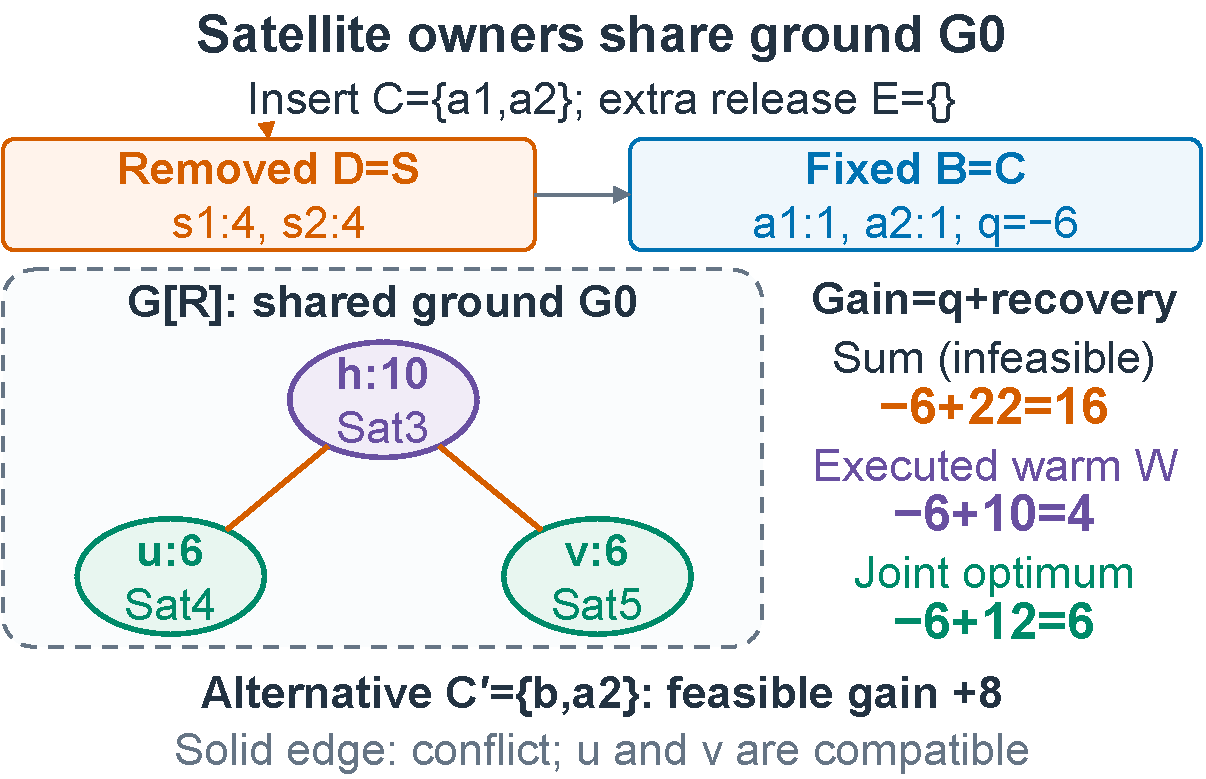
\includegraphics[width=\columnwidth]{v4_figures/residual_schematics/problem_joint_recovery.pdf}
  \caption{Constructed contact example with satellite ownership. Inserting $C$ displaces $D=S$ and fixes $B$, giving $q=-6$. Separate owner recoveries sum to $22$ but conflict on ground G0. All three shared greedy rules return $W=\{h\}$, worth $10$; the compatible joint pair $\{u,v\}$ is worth $12$. Independent addition incorrectly prefers $C$ to the feasible alternative $C'$ with gain $8$; joint recovery reverses this choice. This is a mathematical illustration, not an experimental result.}
  \label{fig:problem-joint-recovery-v4}
\end{figure}


Learning already guides decisions inside combinatorial solvers and selects
subproblems for classical repair~\cite{gasse2019branching,li2021delegate}.
Our focus is the joint recovery value of coordinated adjustments under a
complete decision-time budget. Each action fixes a base schedule and induces
an eligible recovery graph. We represent the remaining alternatives through
their conflicts, resource factors, weights, and observed warm-start
membership. The representation is action-conditioned through this induced
scope; it does not require learning the known immediate gain. Crucially,
every policy first executes a common greedy recovery. The learner estimates
additional joint recoverability between this actual feasible lower value and
a structural upper bound. Sparse fractional occupancies expose competition
among replacements inside that interval; the execution kernel supplies
actual memberships and enforces feasibility.

Finite recovery also depends on how much work the executor receives and
what it has already recovered. We separate these quantities in a factorized
predictor: one structural encoding is shared across requests with the same
recovery graph, factors, and actual warm start, while small heads condition
on the native workpoint and remaining allowance. The immediate gain enters
as an exact final offset. The controller uses these predictions to allocate
paid finite solver calls and retains only validated improvements. Changing
the observed warm start changes the structural input; predictions never
supply an unexecuted recovery as their own warm start.

The paper develops three mechanisms for testing this approach:
\begin{itemize}
  \item A warm-anchored joint recovery predictor that separates a shared,
  already executed greedy value from possible additional recovery, using
  conflicts, resource factors and actual warm membership.
  \item An execution-aligned supervision protocol that compares actual
  finite outcomes from the same state, retaining signed gains, returned
  memberships, failures, and late outcomes.
  \item A factorized finite-call allocator and complete-cost comparison
  protocol covering the declared classical portfolio and matched structural,
  supervision, and warm-start controls.
\end{itemize}

The primary criterion is the objective of the feasible schedule finally
validated and returned within a common total allowance $D$. Proposals,
representation preparation, inference, repair, and final validation are all
charged; a late return receives the original incumbent for this criterion.
We distinguish an improvement available internally before $D$ from timely
return. The completed evaluation covers controlled
coupling graphs and interval-resource scheduling graphs, together with
separate profiles of published solvers on original public graph tasks.
These public profiles establish solver behavior and execution costs;
they do not establish transfer of our learned policy. The central question is whether joint recovery
structure provides useful allocation information beyond strong inexpensive
priorities when every policy pays the same complete decision cost.
The evidence separates the usefulness of the recovery target from the
performance of this particular allocator: finite recovery remains available,
but preparation and caller latency can dominate small decision budgets.
